%%\documentclass[t]{beamer}
\documentclass[t,handout]{beamer}

\usepackage{graphicx}
\usepackage{pgf}
\usepackage{epsfig}
\usepackage{psfrag}
\usepackage[english]{babel}
\usepackage{hyperref}

\usepackage{listings}
\usepackage{courier}
\usepackage{color}

\lstset{
	language=Ruby,
	basicstyle=\footnotesize\ttfamily\color{black},
	commentstyle = \footnotesize\ttfamily\color{red},
	keywordstyle=\footnotesize\ttfamily\color{blue},
	stringstyle=\footnotesize\ttfamily\color{black},
%	columns=fixed,
%	numbers=left,    
	numberstyle=\tiny,
	stepnumber=1,
	numbersep=5pt,
	tabsize=1,
	extendedchars=true,
	breaklines=true,            
	frame=b,         
	showspaces=false,
	showtabs=true,
	xleftmargin=6pt,
	framexleftmargin=6pt,
	framexrightmargin=2pt,
	framexbottommargin=4pt,
	showstringspaces=false      
}

\lstloadlanguages{
         Ruby,HTML
}
 %\DeclareCaptionFont{blue}{\color{blue}}

\newcommand{\asgn}{\mbox{$\bf\leftarrow$ }}  %pseudocode assignment stmt
\newcommand{\comt}{\mbox{$\; \rhd$ \ }}  %pseudocode comment

\graphicspath{{images/}} % Figures path - used in graphicx

%\selectcolormodel{cmyk}

\mode<presentation>

\usetheme{Warsaw}

\title[Module 5, Lecture 2]{ECE 495/595 -- Web Architectures/Cloud Computing}
\subtitle{Module 5, Lecture 2: Web Application Security -- Authentication}

\author[\copyright \ 2012 C. C. Lamb]{Christopher C. Lamb}
\date{}
\institute[University of New Mexico]{\large University of New Mexico}

\titlegraphic{
\begin{figure} 

\includegraphics[width = 4in]{ECE-UNM-logo.pdf}
\end{figure}}

\begin{document}

\begin{frame}
\titlepage
\end{frame}

% This command will make the logo appear on all frames excluding the title frame.
\logo{
\includegraphics[width = 0.75in]{UNM.pdf}}

%\begin{frame}
%\frametitle{Overview}
%\tableofcontents 
%\end{frame}

\section{What is Capistrano?}
\begin{frame}
\frametitle{What is Capistrano?}
~\\
\begin{center}
{\bf Capistrano is a distributed system management framework.} \\
\end{center}
It supports: \\
~\\
\begin{small}
\begin{itemize}
\item Distributed deployments.
\item Command distribution.
\item General large-scale system management.
\end{itemize}
\end{small}
\begin{center}
~\\
{\bf So what?}
\end{center}
\end{frame}

\section{Why use it?}
\begin{frame}
\frametitle{Starting out...}

\includegraphics[width = 4in]{cap-app.pdf}
\transfade
\end{frame}

\begin{frame}
\frametitle{...where to put it?}

\includegraphics[width = 4in]{cap-app-srv.pdf}
\transfade
\end{frame}

\begin{frame}
\frametitle{...and how to store stuff?}
\begin{center}
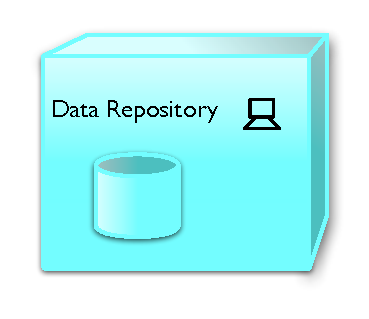
\includegraphics[width = 3in]{cap-data-repo.pdf}
\end{center}
\transfade
\end{frame}

\begin{frame}
\frametitle{...now linking it together...}
\begin{center}
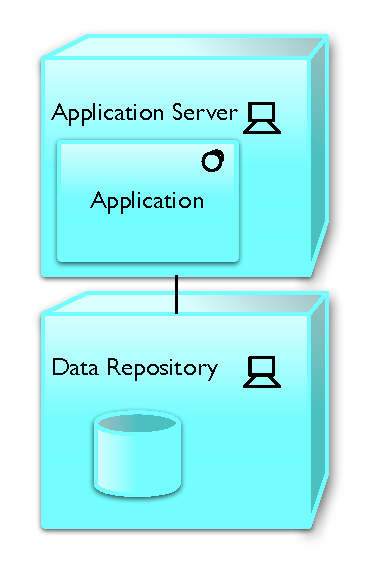
\includegraphics[width = 1.75in]{cap-stack.pdf}
\end{center}
\transfade
\end{frame}

\begin{frame}
\frametitle{...and this is how you manage it.}
\begin{center}
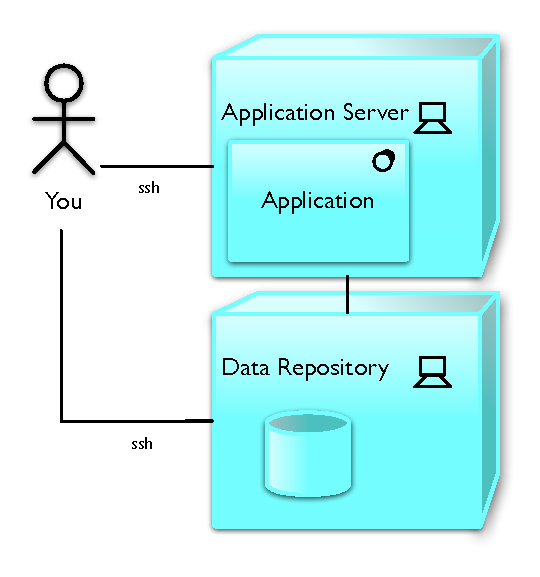
\includegraphics[width = 2.5in]{cap-stack-you.pdf}
\end{center}
\transfade
\end{frame}

\begin{frame}
\frametitle{Is this sufficient?}
Well, probably okay for:
\begin{small}
\begin{itemize}
\item School
\item Departments
\item Small organizations
\end{itemize}
\end{small}
But honestly, not very real world.  Systems with any kind of availability requirements or volume usually have:
\begin{small}
\begin{itemize}
\item More systems
\item Specialized systems
\item More providers
\end{itemize}
\end{small}
\begin{center}
{\bf Really? Well, why not?}
\end{center}
\end{frame}

\begin{frame}
\frametitle{Typical small deployment...}
\begin{center}
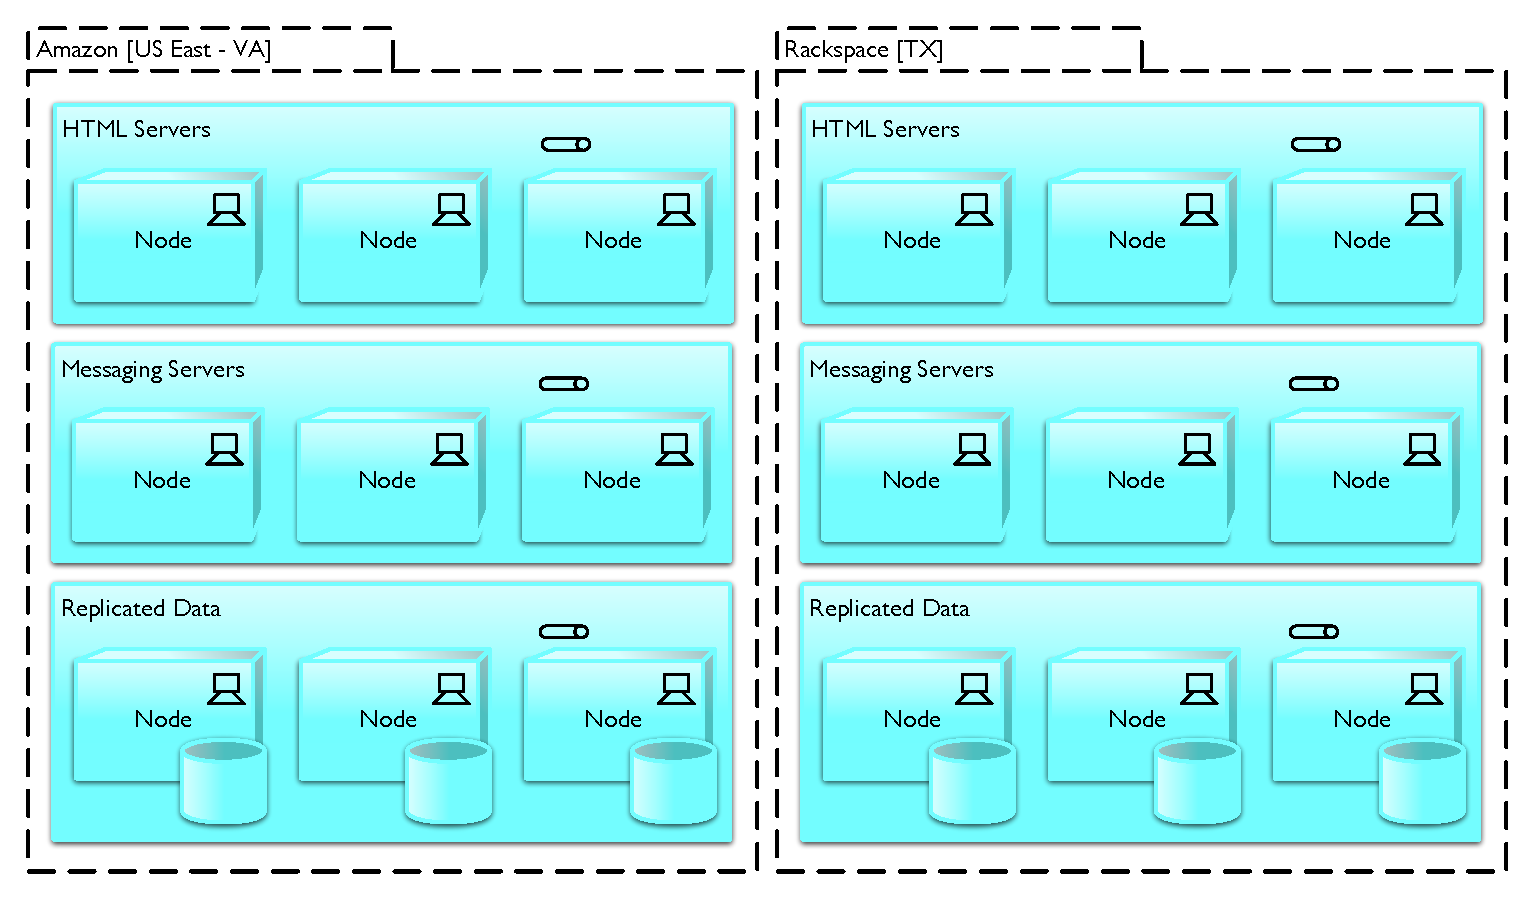
\includegraphics[width = 4in]{cap-distributed.pdf}
\end{center}
\transfade
\end{frame}

\begin{frame}
\frametitle{...and you're responsible for it.}
\begin{center}
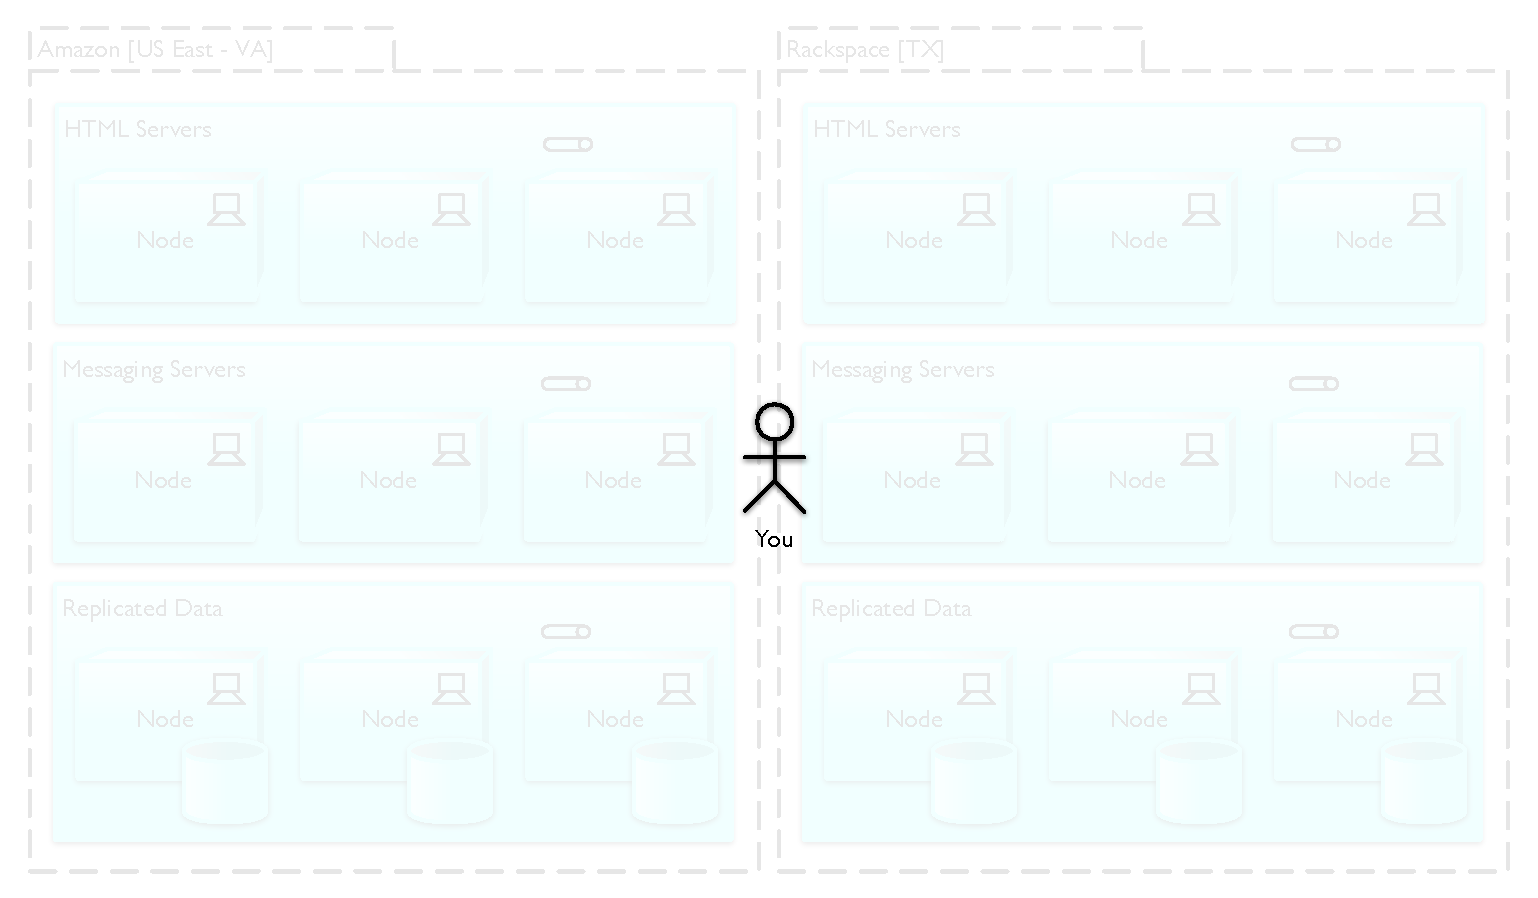
\includegraphics[width = 4in]{cap-distributed-you.pdf}
\end{center}
\transfade
\end{frame}

\begin{frame}
\frametitle{So how do you do it?}
Well, you don't want to log into each system to administer manually.  And why is that?
\begin{small}
\begin{itemize}
\item {\bf Scalability} You don't scale.  Sorry.
\item {\bf Reproducibility}  It's very difficult to recreate the same sequence of actions and configurations across multiple systems, so you'll generally script it.  Which is what Capistrano does, in a distributed way.
\item {\bf Human Error} You make lots of mistakes too.  If you can tell a machine what to do, it'll do a better job than you can.
\end{itemize}
\end{small}
\begin{center}
{\bf So figure out how to tell machines to configure themselves.  Or, use a system built by somebody else to tell machines to configure themselves, like Capistrano.}
\end{center}
\end{frame}

\section{Getting started...}
\begin{frame}
\frametitle{What you need to do first...}
{\bf Capistrano can help you deploy applications, but it needs systems first.} \\~\\
You need to have systems set up and configured for use.
\begin{small}
\begin{itemize}
\item {\bf Chef, Puppet}
\item {\bf Vagrant}
\end{itemize}
\end{small}
They need to have supporting infrastructure installed, like {\bf ruby}, {\bf capistrano}, {\bf bundler}, {\bf rvm}, and {\bf git}.\\~\\
\begin{center}
{\bf Setup isn't turnkey, but future use of Capistrano is.}
\end{center}
\end{frame}


\begin{frame}[fragile]
\frametitle{Starting Out}
Now, install Capistrano on your workstation:\\
\begin{lstlisting}[frame=none,language=Ruby,basicstyle=\scriptsize\ttfamily\color{black},]
$ gem install capistrano
\end{lstlisting}
Or use bundler, with a gem file:
\begin{lstlisting}[frame=none,language=Ruby,basicstyle=\scriptsize\ttfamily\color{black},]
source :rubygems
gem 'capistrano'
\end{lstlisting}
Now initialize the project:
\begin{lstlisting}[frame=none,language=Ruby,basicstyle=\scriptsize\ttfamily\color{black},]
$ cd <project directory>
$ capify .
\end{lstlisting}
This creates, in the project directory, a {\small\tt config} directory containing a {\small\tt deploy.rb} file, and a file in the project root named {\small\tt Capfile}.
%Installation \\
%Project Init\
\end{frame}

\begin{frame}[fragile]
\frametitle{How do these files work?}
{\bf Capfile:}\\
\begin{lstlisting}[frame=none,language=Ruby,basicstyle=\scriptsize\ttfamily\color{black},]
load 'deploy'
load 'config/deploy'
\end{lstlisting}
{\bf config/deploy.rb:}
\begin{lstlisting}[frame=none,language=Ruby,basicstyle=\scriptsize\ttfamily\color{black},]
set :application, "set your application name here"
set :repository,  "set your repository location here"

set :scm, :subversion

role :web, "your web-server here"
role :app, "your app-server here"
role :db,  "your primary db-server here", :primary => true 
role :db,  "your slave db-server here"
\end{lstlisting}
\end{frame}

\begin{frame}[fragile]
\frametitle{What does this give you?}
\begin{lstlisting}[frame=none,language=Ruby,basicstyle=\tiny\ttfamily\color{black},commentstyle=\tiny\ttfamily\color{red}]
$ cap -T
cap deploy                # Deploys your project.
cap deploy:check          # Test deployment dependencies.
cap deploy:cleanup        # Clean up old releases.
cap deploy:cold           # Deploys and starts a `cold' application.
cap deploy:create_symlink # Updates the symlink to the most recently deployed...
cap deploy:migrate        # Run the migrate rake task.
cap deploy:migrations     # Deploy and run pending migrations.
cap deploy:pending        # Displays the commits since your last deploy.
cap deploy:pending:diff   # Displays the `diff' since your last deploy.
cap deploy:restart        # Blank task exists as a hook into which to install...
cap deploy:rollback       # Rolls back to a previous version and restarts.
cap deploy:rollback:code  # Rolls back to the previously deployed version.
cap deploy:setup          # Prepares one or more servers for deployment.
cap deploy:start          # Blank task exists as a hook into which to install...
cap deploy:stop           # Blank task exists as a hook into which to install...
cap deploy:symlink        # Deprecated API.
cap deploy:update         # Copies your project and updates the symlink.
cap deploy:update_code    # Copies your project to the remote servers.
cap deploy:upload         # Copy files to the currently deployed version.
cap deploy:web:disable    # Present a maintenance page to visitors.
cap deploy:web:enable     # Makes the application web-accessible again.
cap invoke                # Invoke a single command on the remote servers.
cap shell                 # Begin an interactive Capistrano session.
\end{lstlisting}
\end{frame}

\begin{frame}[fragile]
\frametitle{Capistrano is Biased}
Nice! But Capistrano was developed expressly to deploy distributed Rails applications and carries baggage around from this heritage.\\~\\

Unless you're deploying Rails, you'll want to get around this --- {\bf railsless-deploy} to the rescue!
\begin{lstlisting}[frame=none,language=Ruby,basicstyle=\scriptsize\ttfamily\color{black},commentstyle=\tiny\ttfamily\color{red}]
$ gem install railsless-deploy
\end{lstlisting}
Or add to your Gemfile:
\begin{lstlisting}[frame=none,language=Ruby,basicstyle=\scriptsize\ttfamily\color{black},commentstyle=\tiny\ttfamily\color{red}]
...
gem 'railsless-deploy'
...
\end{lstlisting}
Other plugins include {\small\tt bundler/capistrano} and {\small\tt rvm-capistrano}.
\end{frame}

\begin{frame}
\frametitle{Other Useful Plug-ins}
You'll want to pre-install {\bf bundler} and {\bf rvm} these on the system you're using. Why?
\begin{small}
\begin{itemize}
\item {\bf bundler} will ensure that your bundles are correctly installed.  Remember you installed bundler in the base image? this also installs {\small\tt bundler/capistrano}, which is what you use to integrate bundler.
\item {\bf rvm} is more than just a gem, so it's out of {\bf bundler}'s league.  A typical {\bf rvm} install in your base image will suffice.  After RVM is installed you can install {\small\tt rvm-capistrano} with {\bf bundler} or via the command line.
\end{itemize}
\end{small}
\begin{center}
{\bf Now let's try this with a real system.}
\end{center}
\end{frame}

\section{...Getting on with it...}
\begin{frame}
\frametitle{A Content Delivery Network}
\begin{center}
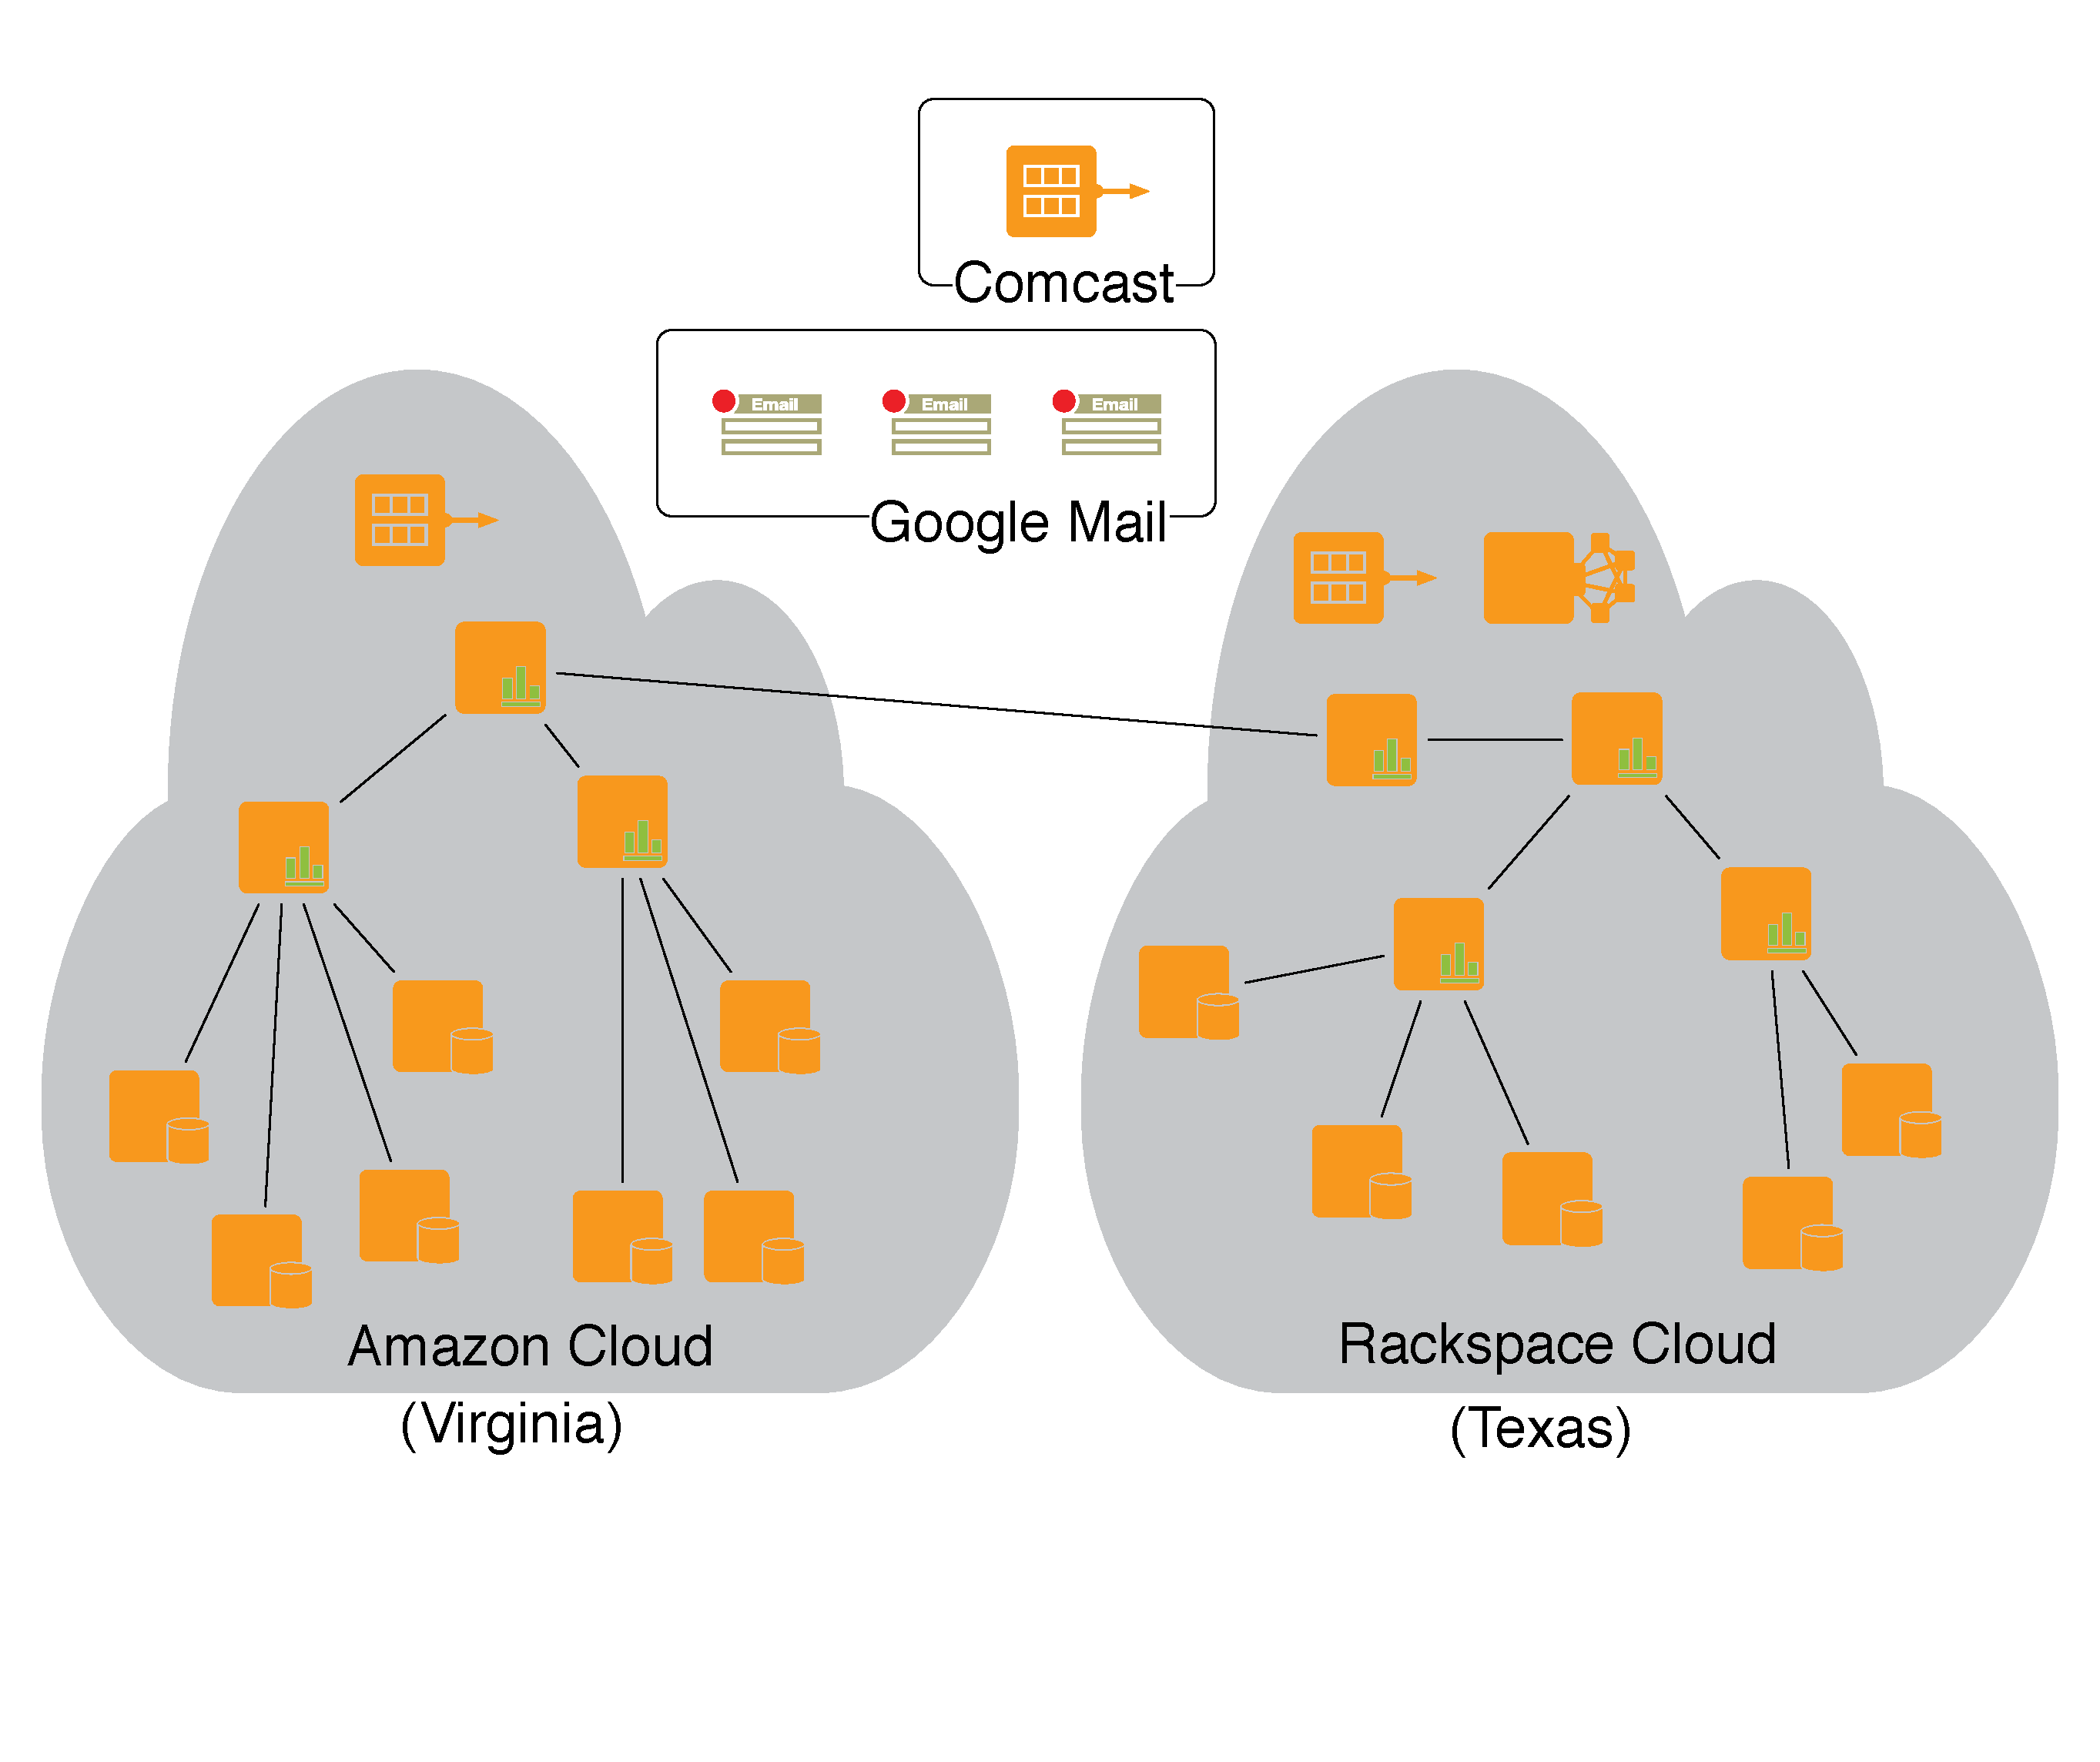
\includegraphics[width = 3.5 in]{hierarchical-clouds.pdf}
\end{center}
\end{frame}

\begin{frame}
\frametitle{How do we support this?}
This has 23 systems across 2 cloud infrastructure providers and integral external services.\\~\\

What tools do we use?
\begin{small}
\begin{itemize}
\item {\bf Base Tooling} --- Ruby, Bundler, RVM
\item {\bf Deployment} --- Capistrano
\item {\bf SCM} --- Git
\item {\bf HTTP Services} ---  S3, EC2, Rackspace Servers
\end{itemize}
\end{small}
\end{frame}

\begin{frame}[fragile]
\frametitle{Capfile}
First, the Capfile: \\
\begin{lstlisting}[frame=none,language=Ruby,basicstyle=\scriptsize\ttfamily\color{black},commentstyle=\scriptsize\ttfamily\color{red}]
require 'rubygems'         # Loading gem support
require 'railsless-deploy' # Loading railsless operation

# Loading vendor supplied plugins
Dir['vendor/gems/*/recipes/*.rb',
    'vendor/plugins/*/recipes/*.rb'].each do |plugin| 
  load(plugin) 
end

load 'config/deploy' # loading deployment tasks
\end{lstlisting}
Why are we altering this file, and not just the {\small\tt config/deploy.rb} file?\\~\\
We need to load the {\small\tt railsless-deploy} support prior to the {\small\tt config/deploy} targets.
\end{frame}

\begin{frame}[fragile]
\frametitle{config/deploy.rb}
Now, the deployment configuration:
\begin{lstlisting}[frame=none,language=Ruby,basicstyle=\scriptsize\ttfamily\color{black},commentstyle=\scriptsize\ttfamily\color{red}]
require 'bundler/capistrano' # Bundler support
require 'rvm/capistrano' # RVM support

require 'yaml' # YAML, for loading config info into S3
require 'aws-sdk' # Support for Amazon S3 APIs (and others)

set :rvm_ruby_string, '1.9.3' # The ruby version we'll use

ssh_options[:keys] = ['etc/pod.pem'] # Amazon key file

# Use GIT, and use this repository with this branch
set :scm, :git
set :repository,  'https://github.com/cclamb/overlay.git'
set :branch, 'final'

set :application, 'content-network' # Application name
\end{lstlisting}
\end{frame}

\begin{frame}[fragile]
\frametitle{config/deploy.rb}
Now, the deployment configuration:
\begin{lstlisting}[frame=none,language=Ruby,basicstyle=\scriptsize\ttfamily\color{black},commentstyle=\scriptsize\ttfamily\color{red}]
# The credentials to use; not maintained in Github
creds_file_name = 'etc/creds.yaml'

# The credentials are formatted in YAML.
creds = YAML::load File::open(creds_file_name)

# This is the format of the YAML file.
msg =<<EOF
Submitted credentials are:
  rackspace password: #{creds['rackspace']['password']}
  amazon access key: #{creds['amazon']['access_key']}
  amazon secret key: #{creds['amazon']['secret_key']}
EOF
puts msg

# Configuring SUDO and deploy locations.
set :use_sudo, false
set :deploy_to, '~'
\end{lstlisting}
\end{frame}

\begin{frame}[fragile]
\frametitle{config/deploy.rb}
Setting credentials and keys:
\begin{lstlisting}[frame=none,language=Ruby,basicstyle=\scriptsize\ttfamily\color{black},commentstyle=\scriptsize\ttfamily\color{red}]
# Setting some credentials for Rackspace.
set :user, 'overlay'
set :password, creds['rackspace']['password']

# Setting the keys for Amazon.
access_key = creds['amazon']['access_key']
secret_key = creds['amazon']['secret_key']
AWS.config \
  :access_key_id => access_key, \
  :secret_access_key => secret_key
\end{lstlisting}
Why do we have so many keys? Remember the PEM file?\\~\\
The PEM file contains keys for {\bf SSH}, the access and secret keys are used to authenticate into Amazon's infrastructure.
\end{frame}

\end{document}


